\pdfoutput=1
\section{Framework Setup}\label{sec: setup}
We summarize 2D-MRA systems and the relation between frequency domain partition and sublattice of $\mathbb{Z}^2$ with critical downsampling following \cite{yin2014orthshear}.

\subsection{Notations and conventions}
Throughout this paper, we use upper case bold font for matrices $(e.g.\;\V{A},\V{B})$, lower case bold font for vectors $(e.g.\;\V{a},\V{b})$ and upper case italics for subsets $(e.g.\;C_1,\,C_2)$ of the frequency domain. We denote the conjugate transpose of a matrix $\V{A}$ by $\V{A}^*$. For $\V{a}$ in a $d$-dimensional vector space over $\mathbb{F}$, we use the convention $\V{a}\in\mathbb{F}^{d\times 1}$ and $\V{a}^*$ for its conjugate row vector. 

We adopt conventions in scientific computing programs and packages. For matrices and vectors, the indexing of rows and columns starts with zero. For the axes of the frequency plane, we denote the vertical axis as $\omega_1$-axis with values increasing from top to bottom and the horizontal axis as $\omega_2$-axis with values increasing from left to right, e.g. Figure \ref{fig: partition}.

\subsection{Multi-resolution analysis and sublattice sampling}
In an MRA, given a scaling function $\phi\in L^2(\mathbb{R}^2)$, such that $\Vert\phi\Vert_2=1$,
the base approximation space is defined as $V_0 = \overlinespace{span\{\phi_{0,\boldsymbol{k}}\}}_{\boldsymbol{k}\in\mathbb{Z}^2}$, where $\phi_{0,\boldsymbol{k}} = \phi(\boldsymbol{x}-\boldsymbol{k})$. If $\langle \phi_{0,\boldsymbol{k}},\phi_{0,\boldsymbol{k'}}\rangle = \delta_{\boldsymbol{k,k'}}$, then $\{\phi_{0,\boldsymbol{k}}\}$ is an orthonormal basis of $V_0$. In addition, $\phi$ is associated with a scaling matrix $\mathbf{D}\in\mathbb{Z}^{2\times 2}$, such that the dilated scaling function
 $\phi_1(\boldsymbol{x}) = |\mathbf{D}|^{-1/2}\phi(\mathbf{D}^{-1}\boldsymbol{x})$ is a linear combination of $\phi_{0,\boldsymbol{k}}$.
Equivalently, $\exists\,m_0(\boldsymbol{\omega}) = m_0(\omega_1,\omega_2)$, $2\pi-$periodic in $\omega_1,\omega_2$, s.t. in the frequency domain
\begin{align}\label{eq: m0}
\widehat{\phi}(\mathbf{D}^T\boldsymbol{\omega}) = m_0(\boldsymbol{\omega})\widehat{\phi}(\boldsymbol{\omega}).
\end{align}
The recursive expression \eqref{eq: m0} of $\widehat{\phi}(\V{\omega})$ implies that
\begin{align}\label{eq: phi-m0}
\textstyle \widehat{\phi}(\boldsymbol{\omega}) = (2\pi)^{-1}\prod_{k=1}^{\infty}m_0(\mathbf{D}^{-k} \boldsymbol{\omega}),
\end{align}
where we have implicitly assumed that $\phi\in L^1(\mathbb{R}^2)$ and $\int\phi\,dx = 1$ (which follows from the other constraints if $\phi$ has some decay at $\infty$).
\\[.2em]
Let $\phi_{l,\boldsymbol{k}} = \phi(\V{D}^{-l}\boldsymbol{x}-\boldsymbol{k})$
and $V_l = \overlinespace{span\{\phi_{l,\boldsymbol{k}};\boldsymbol{k}\in\mathbb{Z}^2\}},\,l\in\mathbb{Z}$ be the nested approximation spaces. Define $W_l$ as the orthogonal complement of $V_l$ with respect to $V_{l-1}$ in MRA. 
Suppose there are $J$ wavelet functions $\psi^j\in L^2(\mathbb{R}^2)$, {\small $1 \leq j \leq J$}, and $\mathbf{Q}\in\mathbb{Z}^{2\times2}$, s.t.
\begin{align*}
\hspace{-1em} W_l = \bigcup_{j=1}^J W_l^j = \bigcup_{j=1}^J \overline{span\{\psi^j_{l,\boldsymbol{k}};\boldsymbol{ k}\in \mathbf{Q}\mathbb{Z}^2\}}= \bigcup_{j=1}^J \overline{span\{\psi^j(\mathbf{D}^{-l}\boldsymbol{x-k});\boldsymbol{ k}\in \mathbf{Q}\mathbb{Z}^2\}},
\end{align*}
 an $L$-level multi-resolution system with base space $V_0$ is then spanned by
 \begin{align}\label{eq: MRA}
 V_L\oplus\,\bigoplus_{l=1}^L\Big(\bigcup_{j=1}^J\, W_l^j\Big) =
 \{\phi_{L,\boldsymbol{k}}\,,\psi^j_{l,\boldsymbol{k'}}\,, \, {\small 1\leq l \leq L,\, \boldsymbol{k}\in \mathbb{Z}^2,\,\boldsymbol{k'}\in \mathbf{Q}\mathbb{Z}^2,\,1\leq j \leq J\}}.
\end{align}  
%In particular, we set $\mathbf{D} = \mathbf{D_2}\doteq\bigl(\begin{smallmatrix} 2&0\\0&2\end{smallmatrix}\bigr)$ and $\mathbf{Q}\doteq\bigl(\begin{smallmatrix} 1&1\\-1&1\end{smallmatrix}\bigr)$.
As $W_1\subset V_0$, each rescaled wavelet $\psi^j(\mathbf{D}^{-1}\cdot)$ is also a linear combination of $\phi_{0,\boldsymbol{k}}$, so that there exists $m_j$ analogous to $m_0$
satisfying 
\begin{align}\label{eq: mj}
\widehat{\psi}^j(\mathbf{D}^T\boldsymbol{\omega}) = m_j(\boldsymbol{\omega})\widehat{\phi}(\boldsymbol{\omega}),\hspace{1cm} 1\leq j \leq J.
\end{align}
%In this specific construction of MRA,
% the scaling function $\phi$ and all the wavelet functions $\psi^j$ share the same scaling matrix $\mathbf{D}$, yet the family of shifted $\phi_{\boldsymbol{k}}$ is defined on $\mathbb{Z}^2$, whereas the family of shifted $\psi^j_{\boldsymbol{k}}$ is defined on a sub-integer lattice $\mathbf{Q}\mathbb{Z}^2$. Hence 
% the corresponding subsampling matrix of $\phi_{1,\boldsymbol{k}}$ is $\mathbf{D}$ and that of $\psi^j_{1,\boldsymbol{k}}$ is $\mathbf{QD}$, the dyadic quincunx subsample (see the right panel in Fig.\ref{fig: partition}), as in \cite{durand2007}. 
% We haven't yet imposed any condition on this MRA, or equivalently, on $m-$functions and the subsampling matrices $\mathbf{D}$ and $\mathbf{Q}$; this comes next.


\subsection{Frequency domain partition and critical downsampling}\label{subsec: frequency partition}

%critical downsampling thus depends only on the subsampling matrices $\mathbf{D}$ and $\mathbf{Q}$. The space decomposition structure $V_0 = V_1\bigoplus W_1$ in MRA and \eqref{eq: m0}, \eqref{eq: mj} require consistency between the $m-$functions and the subsampling matrices $\mathbf{D}$ and $\mathbf{Q}$. 

\begin{figure}[!t]
\centering
\begin{minipage}[c]{.35\textwidth}
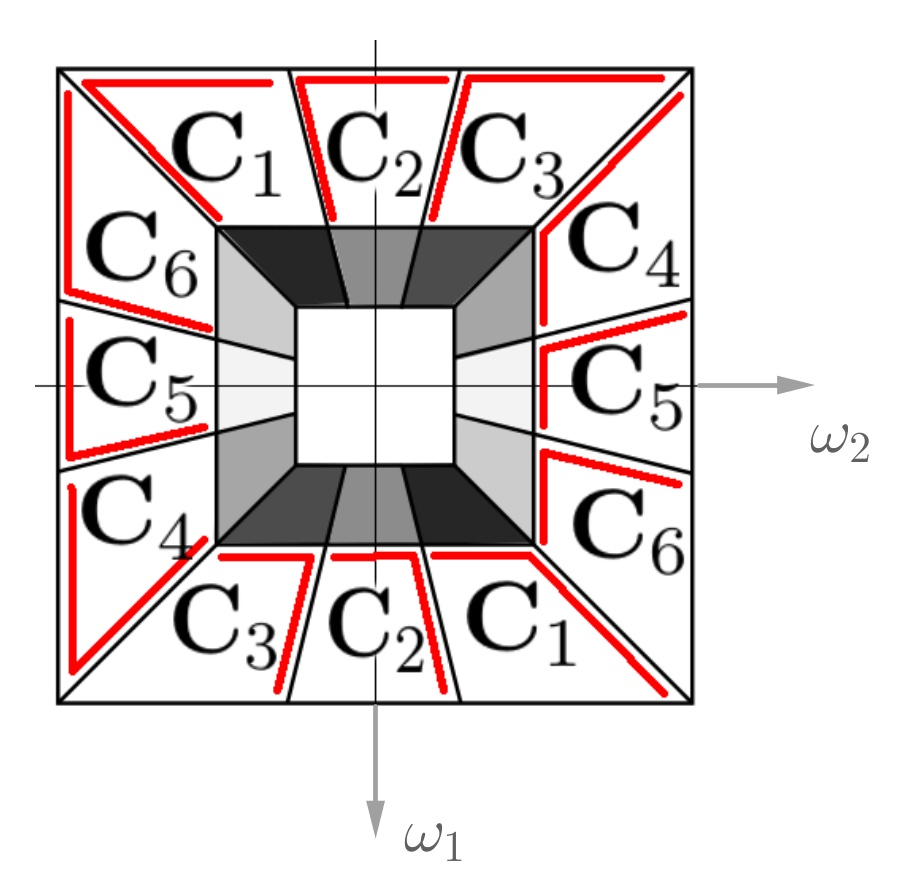
\includegraphics[width=\textwidth]{shannon-marked-wcoord.jpg}
\end{minipage}\hspace*{3em}
\begin{minipage}[c]{.25\textwidth}
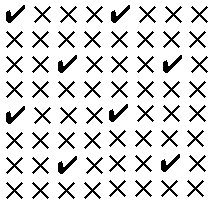
\includegraphics[width=\textwidth]{sublattice-2.jpg}
\vspace*{1em}
\end{minipage}
\caption{Left: partition of $S_0$ and boundary assignment of $C_j$, $j = 1,\cdots,6$ (each $C_j$ has boundaries indicated by red line segments), Right: dyadic quincunx sublattice. Note that the $\omega_1$-axis is vertical and the $\omega_2$-axis is horizontal by our convention.}
\label{fig: partition}
\vspace*{-5mm}
\end{figure}

%\begin{mydef}
%If $\mathcal{L}$ is the lattice generated by $\boldsymbol{a}_1,\boldsymbol{a}_2$, i.e. $\mathcal{L} = \sum_{i=1,2}k_i\boldsymbol{a}_i,\,k_i\in\mathbb{Z}$,the {\bf reciprocal lattice} $\mathcal{L}^*$ of $\mathcal{L}$ is the lattice generated by the vectors $\boldsymbol{b}_1,\boldsymbol{b}_2$, s.t. $\boldsymbol{b}_i^T\boldsymbol{a}_j = 2\pi\delta_{ij}$. 
%\end{mydef}

%\begin{mydef}
%Given a lattice $\mathcal{L}$, a {\bf fundamental domain} $S$ in $\mathbb{R}^2$ with respect to $\mathcal{L}$, denoted as $S = \mathbb{R}^2/\mathcal{L}$, is a subset of $\mathbb{R}^2$, such that $\bigcup_{l\in\mathcal{L}}(S+l) = \mathbb{R}^2$ and $S\cap(S+l)=\varnothing,\,\forall l\in\mathcal{L}\setminus\{\mathbf{0}\}$.
%A set $S$ is a {\bf frequency support} of $\mathcal{L}$ if $S = \mathbb{R}^2/\mathcal{L}^*$.
%\end{mydef}
%Furthermore, each sub-lattice $\mathcal{L}$ of $\mathbb{Z}^2$ is associated with a set of shifts $\Gamma, \, s.t. \bigcup_{\V{\gamma}\in\Gamma}\mathcal{L}+\V{\gamma} = \mathbb{Z}^2$ and $|\Gamma| = |\mathbb{Z}^2/\mathcal{L}|$.

Consider the canonical frequency square, $S_0 = [-\pi,\pi)\times[-\pi,\pi)$ associated with the lattice $\mathcal{L} = \mathbb{Z}^2$. 
%Due to \eqref{eq: m0} and \eqref{eq: mj}, this is equivalent to $S_0=\bigcup_{0\leq j\leq J} supp(m_j\vert_{S_0})$.That is, 
For $L=1$, the 1-level decomposition \eqref{eq: MRA} together with \eqref{eq: m0} and \eqref{eq: mj} implies that the union of the support of $m_j,\,0\leq j\leq J$ covers $S_0$.
Furthermore, there exist $C_j\subset supp(m_j), 0\leq j\leq J,$ such that they form a partition of $S_0$; conversely, given a partition $C_j$ of $S_0$, we may construct an MRA where $m_j$ are ``mainly" supported on $C_j$ (this will become more explicit in Section \ref{subsec: discontinuity}).
%, and it is natural to take $C_j$ as the main support of $m_j$.
To build an orthonormal basis with good directional selectivity, we choose the partition of $S_0$ shown in the left of Figure \ref{fig: partition}, which is the same for Example B in \cite{durand2007}\textcolor{blue}{, or equivalently the frequency partition in the coarsest level of the least redundant shearlet system} \cite{kutyniok2012digital}. In this partition, $S_0$ is divided into a central square $C_0 = \bigl(\begin{smallmatrix} 2&0\\0&2\end{smallmatrix}\bigr)^{-1}S_0$ and a ring: the ring is further cut into six pairs of directional trapezoids $C_j$ by lines passing through the origin with slopes $\pm 1, \pm 3$ and $\pm \frac{1}{3}$. The central square $C_0$ can be further partitioned in the same way to obtain a two-level multi-resolution system, as shown in Figure \ref{fig: partition}. 


%To build our first example, in which $\hat{\phi},\,\widehat{\psi}^j$ are indicator functions in $\mathbb{R}^2$, we consider the case where  and we pick $S_0=\mathbb{R}^2/(\mathbb{Z}^2)^*$, . 
%Since $\phi_1,\psi^j_1$ and their shifts span the space $V_0$, $supp(\widehat{\phi}_1)$ and $supp(\widehat{\psi}^j)$, together, should thus cover $S_0$. Due to \eqref{eq: m0} and \eqref{eq: mj}, this is equivalent to $S_0=\bigcup_{0\leq j\leq J} supp(m_j\vert_{S_0})$. That is, if $C_j,\,{\small 0\leq j\leq J}$ are the main support of $m_j,\,0\leq j\leq J$ respectively, then they form a partition of $S_0$. An non-uniform admissible partition is defined as follows,

%\begin{mydef}
%$C_j, 0\leq j\leq J$ is an {\bf admissible} partition of $S_0$ if and only if $\exists \mathbf{D}, \mathbf{Q}\in\mathbb{Z}^{2\times 2}$, s.t. the low frequency piece $C_0 = \mathbb{R}^2/(\mathbf{D}\mathbb{Z}^2)^*,$ and the high frequency pieces $C_j = \mathbb{R}^2/(\mathbf{QD}\mathbb{Z}^2)^*,\,j = 1,\cdots,J$.
%\end{mydef}
In the corresponding MRA generated by \eqref{eq: MRA}, $J=6$ and $\mathbf{D} =\bigl(\begin{smallmatrix} 2&0\\0&2\end{smallmatrix}\bigr)$, and we choose  $\mathbf{Q}$ specifically to be $\bigl(\begin{smallmatrix} 1&1\\-1&1\end{smallmatrix}\bigr)$. Because $ |\mathbf{D}|^{-1} + J|\mathbf{QD}|^{-1} = 1/4 + 6/ (2\cdot 4) = 1$, the corresponding MRA generated by \eqref{eq: MRA} achieves critical downsampling(\cite{durand2007}). The scaling matrix of $\psi^j$ is $\V{QD}=\bigl(\begin{smallmatrix} 2 & 2\\-2 & 2\end{smallmatrix}\bigr)$, which corresponds to downsampling on the dyadic quincunx sublattice $\V{QD}\mathbb{Z}^2$ (see the right panel in Figure \ref{fig: partition}), as in \cite{durand2007}. 

%\noindent{\it Remark.}
%The dyadic quincunx subsampling $\V{QD}$ is not ideal for $\psi^2$ with frequency support on  $C_2$ that characterizes horizontal features. However, we can adapt the subsampling lattice $\V{QD}\mathbb{Z}^2$ by shearing it. In particular, let $\V{S} = \bigl(\begin{smallmatrix} 1&0\\1&1\end{smallmatrix}\bigr)$ be the shearing matrix, then $\V{SQD}\mathbb{Z}^2 = \bigl(\begin{smallmatrix}2 & 2\\ 0 & 4\end{smallmatrix}\bigr) \mathbb{Z}^2= \bigl(\begin{smallmatrix}2 & 0\\0 & 4\end{smallmatrix}\bigr)\mathbb{Z}^2$, a sublattice where the horizontal subsampling factor is twice of the vertical one. Since $|\V{S}|=1$, the critical downsampling property still holds and all the analysis in the rest of this paper stays the same. For $\psi^5$, we can shear $\V{QD}\mathbb{Z}^2$ by $\V{S}' = \bigl(\begin{smallmatrix} 1 & -1\\ 0 & 1\end{smallmatrix}\bigr)$ to obtain $\V{S}'\V{QD}\mathbb{Z}^2 = \bigl(\begin{smallmatrix} 4 & 0\\0 & 2\end{smallmatrix}\bigr)\mathbb{Z}^2$.

This downsampling scheme is compatible with $C_j$. Consider two sets of shifts in the frequency domain $\Gamma_0= \{\V{\pi}_i,\, i = 0,2,4,6\}$ and $\Gamma_1 = \{\V{\pi}_i,\, i = 0,1,\cdots,7\}$, where {\small $\V{\pi}_0 = (0,0), \V{\pi}_1 = (\pi/2,\pi/2), \V{\pi}_2 = (\pi,0),\V{\pi}_3 = (-\pi/2,\pi/2), $ $\V{\pi}_4 = (0,\pi), \V{\pi}_5 = (\pi/2,-\pi/2),\V{\pi}_6 = (\pi,\pi), \V{\pi}_7=(-\pi/2,-\pi/2)$}. $\Gamma_0$ and $\Gamma_1$ characterize the sublattices $\V{D}\mathbb{Z}^2$ and $\V{QD}\mathbb{Z}^2$ respectively by
$\sum_{\V{\pi}\in\Gamma_0}e^{i\V{\alpha}^\top\V{\pi}} = |\Gamma_0| \, \mathbbm{1}_{\V{D}\mathbb{Z}^2}(\V{\alpha})$ and $ \sum_{\V{\pi}\in\Gamma_1}e^{i\V{\alpha}^\top\V{\pi}} = |\Gamma_1| \, \mathbbm{1}_{\V{QD}\mathbb{Z}^2}(\V{\alpha})$, where $\mathbbm{1}$ is the indicator function. 
We observe that each $C_j$ forms a tiling of $S_0$ under the shifts associated with the sublattice where the coefficients of $\psi^j$ are downsampled:
% Each $C_j$ together with its shifts form a tiling of $S_0$, i.e.
\begin{align}\label{eq: tiling}
S_0 = \bigcup_{\V{\pi}\in\Gamma_1}\left(C_j + \V{\pi}\right) = \bigcup_{\V{\pi}\in\Gamma_0}\left(C_0 + \V{\pi}\right),\quad j = 1,\cdots,6.
%\mathbb{R}^2/(\mathbb{Z}^2)^*=\bigcup_{\V{\pi}\in\Gamma_0}\left(\mathbb{R}^2/(\V{D_2}\mathbb{Z}^2)^* %+ \V{\pi}\right)
%=\bigcup_{\V{\pi}'\in\Gamma_1}\left(\mathbb{R}^2/(\V{QD_2}\mathbb{Z}^2)^* + \V{\pi}'\right),
\end{align}
%where%then $\mathbf{D_2}\mathbb{Z}^2$ is associated with the set of shifts 
%$\Gamma_0= \{\V{\pi}_i,\, i = 0,2,4,6\}$ and %$\mathbf{QD_2}\mathbb{Z}^2$ is associated with 
%$\Gamma_1 = \{\V{\pi}_i,\, i = 0,1,\cdots,7\}$.
Alternatively, we say that $\{\,C_j,\, j = 0,\cdots,6\,\}$ is an {\it admissible} partition of $S_0$ with respect to the dyadic quincunx downsampling scheme.
%This partition is admissible and corresponds to $\mathbf{D} = \mathbf{D_2}\doteq\bigl(\begin{smallmatrix} 2&0\\0&2\end{smallmatrix}\bigr)$ and $\mathbf{Q}:=\bigl(\begin{smallmatrix} 1&1\\-1&1\end{smallmatrix}\bigr)$. The wavelet coefficients are taken on the dilated quincunx sub-lattice $\mathbf{QD_2}\mathbb{Z}^2$ (see the right panel in Fig.\ref{fig: partition}).
%In addition, $|\mathbf{D_2}| = 4,\,|\mathbf{Q}| = 2$ so that $1/4 + 6/ (2\cdot 4) = 1$, and the system is critical downsampling.
The admissible property guarantees the existence of orthonormal bases consisting of directional filters on the dyadic quincunx sublattice with frequency support in $C_j$.